%%%%%%%%%%%%%%%%%%%%%%%%%%%%%%%%%%%%%%%%%%%%%%%%%%%%%%%%%%%%%%%%%%%%%%%%%%%
%
%    phase1-AR.tex  (use only for Archival Research and Theory proposals; 
%                     use phase1-GO.tex for General Observer and Snapshot
%                     proposals and phase1-DD.tex for GO/DD proposals).
%
%    HUBBLE SPACE TELESCOPE
%    PHASE I ARCHIVAL & THEORETICAL RESEARCH PROPOSAL TEMPLATE 
%    FOR CYCLE 21 (2013)
%
%    Version 1.0, December  1, 2012.
%
%    Guidelines and assistance
%    =========================
%     Cycle 21 Announcement Web Page:
%
%         http://www.stsci.edu/hst/proposing/docs/cycle21announce 
%
%    Please contact the STScI Help Desk if you need assistance with any
%    aspect of proposing for and using HST. Either send e-mail to
%    help@stsci.edu, or call 1-800-544-8125; from outside the United
%    States, call [1] 410-338-1082.
%
%%%%%%%%%%%%%%%%%%%%%%%%%%%%%%%%%%%%%%%%%%%%%%%%%%%%%%%%%%%%%%%%%%%%%%%%%%%

% The template begins here. Please do not modify the font size from 12 point.

\documentclass[12pt]{article}
\usepackage{phase1,hyperref,graphicx,color}

\newcommand{\documentname}{\textsl{AR Proposal}}
\newcommand{\project}[1]{\textsl{#1}}
\newcommand{\HST}{\project{HST}}
\newcommand{\WFC}{\project{WFC3}}
\newcommand{\MAST}{\project{MAST}}
\newcommand{\dd}{\mathrm{d}}

\newcommand{\bvec}[1]{\textbf{\textit{#1}}}

\begin{document}

%   1. SCIENTIFIC JUSTIFICATION
%       (see Section 9.1 of the Call for Proposals)
%
%
\justification          % Do not delete this command.

With weak lensing surveys, high-redshift galaxy science, and exoplanet
discovery and characterization, the requirements on imaging
calibration are becoming extremely severe.  At the same time,
next-generation projects like \project{JWST}, \project{Euclid}, and
\project{WFIRST} are being designed with very strong budget and
observing-time pressure on calibration programs: We want as much of
the data in ``science'' mode as possible.  One paradox of calibration
programs is that although they incur significant operational overheads
(especially for projects like \project{Euclid} performing large
solid-angle surveys with strict cadence requirements), it is
nonetheless the case the vast majority of the \emph{photons} detected
by the infrared detectors will be detected in the science frames, not
the calibration frames.  The science frames themselves therefore
contain enormous stores of information about calibration.  Unlocking
this information is the goal of the group of methods known as
\emph{self-calibration}.  In this \documentname, we propose to develop
a completely new kind of self-calibration that has the potential to
deliver precise, fine-scale imaging calibration.  We propose to apply
the new methods to the entire body of \WFC\ IR-channel data available
in \MAST.  Our deliverables will be new \WFC\ flat-field maps and the
code that generated them.

Precise calibration of the detector in an astronomical imaging camera
is not trivial---and it is only harder if it is in space.
Fundamentally, the sensitivity of the device must be calibrated with
incident photons; no artificial light source is available; even if an
artificial source \emph{were} available, it could not be designed to
illuminate the device exactly as does a star or other astronomical
source.

The imaging devices of \HST\ (and specifically \WFC) are calibrated by a number of
methods:
\\ $\bullet$ \project{laboratory calibration}: The instrument was illuminated
  in the laboratory pre-flight (\href{http://bit.ly/Xn8OOH}{ISR WFC3
    2008-28}).  In principle this calibration can be
  done perfectly, but \textsl{(a)}~usually the calibration
  illumination does not illuminate the instrument exactly as does an
  in-flight star observation, and \textsl{(b)}~usually the light
  source does not have a completely appropriate SED.  The laboratory
  calibration happens pre-launch, so changes in the instrument through
  launch and in flight cannot be captured, nor can some aspects of in-launch
  environment (loading, temperature, pressure).
\\ $\bullet$ \project{standard stars}: On a regular schedule, well-understood
  standard stars are placed in the instrument focal plane to test the
  on-orbit throughput of the device (e.g.,
  \href{http://bit.ly/Y7wx5v}{ISR WFC3 2009-05}).  These
  observations are key to instrument monitoring, but they don't
  calibrate the device at the pixel level; they provide only overall
  throughput measurements.
\\ $\bullet$ \project{grid test}: The throughput measurements are transferred
  out to the entire device by grid tests, in which standards or a star
  field are stepped over the instrument focal plane (e.g., \href{http://bit.ly/XFdEYW}{ISR WFC3
  2009-39}).  This brings the same astronomical source to many
  different focal-plane positions; it permits relative calibration of
  different parts of the detector. The grid, however, is not dense at
  the pixel level.  The grid test does not provide a pixel-to-pixel
  flat field; it only calibrates the flat on large scales.
\\ $\bullet$ \project{super-flat}: The only in-flight source of
  pixel-to-pixel sensitivity information are the photons detected in
  the sky---the blank parts of the imaging.  These photons can be
  combined (with masking of detected astronomical sources) into a
  pixel-level sensitivity map (\href{http://bit.ly/YJJB2m}{ISR
    WFC3-2011-11}).  Unfortunately, this
  map is a sensitivity to the \emph{sky} not to a \emph{star}: The sky
  has a different SED than any star.  More importantly, the
  uniform-brightness sky illuminates the device differently than any
  star.  This problem is a bigger problem for open-structure
  ground-based telescopes than it is for \HST, but it isn't known to
  be negligible for \HST.  

There is no method---not even any \emph{combination of methods}---that
can be used to do all of \textsl{(1)}~test the calibration of the
detector in-flight, \textsl{(2)}~provide information on pixel-to-pixel
relative sensitivity (small scales), \textsl{(3)}~illuminate the
detector as stars do, and \textsl{(4)}~illuminate with the SED or
color of astronomical sources of interest.  It is possible that these
things don't matter---that every pixel of every \HST\ instrument is
properly calibrated---but it is close to impossible to know with the
calibration data available at present.  That is, if the flat
appropriate to stellar sources is different at fine (pixel-level)
angular scales from the flat appropriate to sky photons, that problem
would not appear strongly in current calibration data.

\textbf{Here we propose to calibrate the \WFC\ IR channel at the pixel
  level using all of the F110W and F160W science data availble in \MAST.}
Importantly, we will build this calibration from the astronomical
sources in the data, \emph{not} the blank-sky parts of the imaging.
By construction, the flats we produce will be built from sources with
astrophysically relevant SEDs.

In general there are two approaches for self-calibration of this kind.
The first---what we might call ``traditional'' self-calibration---is
built on the principle that if the \emph{same object} is observed at
\emph{different focal-plane positions} the inferences made ought to be
independent of focal-plane position.  This kind of self-calibration is
most effective when the observatory obeys calibration-oriented
observing strategies (Holmes et al., 2012,
\href{http://dx.doi.org/10.1086/668656}{PASP, 124, 1219}), and those strategies
involve multiple observations for most sources.  The simplest kind of
self-calibration is the ``grid test'' mentioned above.  The most
ambitious self-calibration was that performed (by the PI and
collaborators) with the entire point-source catalog of the
\project{Sloan Digital Sky Survey} (Padmanabhan et al., 2008,
\href{http://bit.ly/12dPkSh}{ApJ, 674, 1217}).  Traditional
self-calibration (beyond the grid test) is not applicable to most
\HST\ instruments, because sources are rarely observed multiple times,
and when they are it is usually on one of a small number of
small-angle dithers.  Good self-calibration requires a large diversity
of large-angle dithers (Holmes et al., op cit.).

In the second approach---what we might call ``probabilistic''
self-calibration---the fundamental principle is that no \emph{pixel}
will see a \emph{special set of astronomical objects}.  (Of course
this assumption is wrong in important ways, to which we will return
below.  This kind of
self-calibration is applicable in (almost) any observing strategy,
provided that the imager has been used to make \emph{an large
  number of observations}.

In a probabilistic self-calibration, the idea is that any patch of any
image from any exposure in any region of the focal plane ought to be
possible to generate from some kind of reasonable astronomical
``scene'' convolved with the known point-spread function.  Aside from
the differences generated by the variation of the PSF over the
field-of-view, the distribution of possible image patches ought to be
the same in all parts of the device.  In other words, every small
(calibrated) image patch---when the device is properly
calibrated---must display a (very tiny) scene that \emph{could
  possibly be observed} by \HST.  If the calibration parameters get
set to bad values, the observed image patches will contain imprints of
the calibration errors, related to the location on the focal plane
from which they are taken (see Figure).

The simplest possible version of a probabilistic
self-calibration is the construction of the ``super-flat'' in the
current \WFC\ calibration strategy; the super-flat is constructed by
forcing statistics of the pixel values to be constant across the
device.  The most extreme version of probabilistic self-calibration
would be to construct highly informative prior PDFs for astronomical
scenes and find the calibration parameters (and PSF parameters,
perhaps) at which the output images match best those priors!  Here we
propose to do something intermediate, much more ambitious and
informative than the super-flat, but tractable with current \WFC\ data
and computation.

%%%%%%%%%%%%%%%%%%%%%%%%%%%%%%%%%%%%%%%%%%%%%%%%%%%%%%%%%%%%%%%%%%%%%%%%%%%
%   2. ANALYSIS PLAN
%       (see Section 9.6 of the Call for Proposals)
%
\describearchival       % Do not delete this command.
% Enter your analysis plan here.

The goal of our archival analysis is to perform a probabilistic
self-calibration of \WFC\ IR-channel data.  There is a huge range of interesting
and valuable calibration issues to consider, including the static or slowly 
evolving flat, SED dependence, temperature effects, or transients
(e.g., persistence, and the ``snow balls'').  Since our approach is
new and somewhat exploratory, our Analysis Plan is to first focus on
a baseline project, taking advantage of much of the current
knowledge of \WFC\ (e.g., the PSF model).  Once the baseline project is understood
and delivered, we will specify and focus on enhanced deliverables.

\textbf{Our baseline goal is to produce a new, pixel-to-pixel
  flat field model for the \WFC\ IR channel.}
Fundamentally, our method relies on the fact
that many of the sources in the data are stars or compact galaxies, convolved by the PSF at
the location on the detector.  Beyond a simple normalization,
therefore, all stars ought to look similar if the PSF (as a
function of time and position) is well understood, and the
pixel-to-pixel calibration of the instrument is correct.  If, however,
a there are small errors in the pixel-to-pixel flat field, stars whose flux
touches the poorly calibrated pixel will look somewhat distorted (see Figure).

We intend to build a pixel-level, generative model
for the (entirety of the) \WFC\ IR-channel data, under the best current PSF model.  We begin by
taking all $M$ images taken through a filter, dividing up the images into
small patches $D_n$ (baseline will be $5 \times 5$ pixels), $N$ of which contain
significant flux from one or more astronomical sources.  Here, our baseline approach assumes
everything in the \textsl{calwfc3} pipeline to be true, except for the
flat field, which we will infer.  Therefore, the $D_n$ patchs are taken
from home-made \texttt{flt} files (which are generally calibrated but which have had no flat applied), and for
which cosmic-ray and bad pixel masks are known.

Our model for patch $D_n$ is
\begin{eqnarray}
D_n & = & F_n \cdot (S_n \otimes \Psi_n) + \epsilon_n + H_n
\quad 
\end{eqnarray}
where $F_n$ is the tiny relevant patch of the flat, $S_n$ is a high-resolution (tiny) image, $\Psi_n$
is the PSF relevant to the patch, $\epsilon_n$ is a noise
contribution, and $H_n$ includes everything else we are (for now) ignoring.
In short, we model the patch $D_n$ as an underlying astronomical scene
$S_n$ (flux located at a delta function in space for stars, surface
brightness distribution for galaxies) convolved with the
pixel-convolved and pixel-sampled PSF.  Note that the model for $S_n$
will include sources with centroids outside the patch in a large
fraction of patches!  The excess $H_n$ includes both lower order
effects (like problems with bias and zero contributions) and higher order effects
(like persistence).  For our baseline we will mask or ignore such
problems, but will return to these issues as enhanced goals (see below).
Additionally, our baseline project will assume a PSF model across the
detector, from observations of bright stars (e.g.,
\href{http://bit.ly/XFSb1M}{ISR WFC3 2009-37}).  Note the patch $D_n$
has associated metadata (like time, temperature, and location on the
detector).  We will use this to identify the correct portion of the
current flat field model, as well as the correct PSF and noise model
(since, e.g., the PSF is known to vary over time and location).

We will adopt standard \HST\ noise models to generate the distribution
(variance tensor $\sigma_n^2$) for the noise $\epsilon_n$.  In the
probabilistic approaches we will use, we can drop or ignore bad pixels
and cosmic rays by simply treating those pixels as having infinite
variance (or vanishing inverse variance $\sigma_n^{-2}$); these bad
pixels end up with zero weight in all operations.

A critical part of this model involves inference of the underlying
scene $S_n$, which can often be quite complicated.  We plan to start by restricting the $N$ total patches to those whose
scenes are well fit by a background level plus a small number (say one or two) stars, or a single compact
galaxy (well fit, say, by a S\'{e}rsic profile).  After determining
the patches to use for calibration, we can determine the flat field
using standard interference machinery:
\begin{eqnarray}
p(D_n|F,S_n,\epsilon_n) &=& N(F \cdot (S_n \otimes \Psi_n), \sigma_n^2)
\\
p(\bvec{D}|F,{\bf S},{\bf \Psi},{\bf \sigma}) &=& \prod_n^N
p(D_n|F,S_n,\sigma_n) \\
p(F|\bvec{D},{\bf \epsilon}) & \propto & p(\bvec{D}|F,{\bf S},{\bf \Psi},{\bf
  \sigma})\, p(F)\, p({\bf S})\, p({\bf \Psi})
\quad .
\end{eqnarray}
That is---because we can write down a probability for the data given model
parameters---we can infer those model parameters either in a maximum-likelihood
sense or in a sample-from-posterior PDF sense.
Here we have treated the likelihood for individual patches as
Gaussian, under the noise model determined by \textsl{calwfc3}.  The
total likelihood is just the product over all patches.  The posterior
probability of the flat field involves specifying priors over
\textsl{(1)} the flat field, which we will take (at first) to be a
very narrow distribution in flat-field space centered on the the
\textsl{calwfc3} LP flats, \textsl{(2)} a prior over scenes ${\bf S}$,
which we will start by making power-law distribution of stellar
brightnesses and unclustered spatial distributions (which are pretty
good for tiny image patches), and \textsl{(3)} the PSF model which we
will assign as mentioned above, but with some uncertainty.

We plan to deliver (for our baseline) the pixel-to-pixel flat fields
(and software that produces them) for the F110W and F160W filters.  We
are choosing these particular filters since they are the most
heavily used with \WFC\ IR-channel observations, having been used for
1626 and 4149 exposures respectively (as of 2013-02-27) longer than
100~s.  In addition, we choose these filters since they provide a set
of tests with which we can assess the fidelity of our flat fields.
Specifically, we will first examine the consistency of the photometry
of standard stars (gridded across the detector in standard calibration observations).

For end-to-end testing of our delivered flat, Jason
Kalirai (STScI) has volunteered to reprocess \WFC\ observations of 47 Tuc (see
Kalirai et al. 2012, \href{http://dx.doi.org/10.1088/0004-6256/143/1/11}{AJ, 143, 11}),
for which we can examine the
consistency of the Main Sequence of the cluster.  In both cases,
photometry will be performed on the individual dithers, rather than
the drizzled images (which may introduce scatter, depending on the
procedure).  By comparing the results from our flat fields to those
using standard \emph{calwfc3} flats (as well as the flat fields
themselves), \emph{we will produce the first verification of the pixel
  level flat field since the launch of \WFC}.  Beyond this zeroth-level
result from our baseline project, we expect we will learn new ways in
which the calibration can be improved, and we very much hope to provide a scientifically
improved calibration of the IR channel through the F110W and F160W filters.  Currently, the
uncertainty in the flat fields are about $0.5\%$, with a peak-to-peak
variation of $-1.5$ to $+1.6\%$ (see ISR WFC3-2011-11).  We view this
baseline exploratory archival calibration project as a worthwhile step forward
towards next-generation calibration techniques.

The above Analysis Plan includes simplified and
achievable deliverables.
However, we intend to follow this delivery with enhanced-goal projects that
attack increasingly difficult calibration problems:
\\ $\bullet$
There are projects related to time and temperature: The sensitivity
of the device is known to be a function of both temperature and time,
with defects and sensitivity changes appearing during the mission.  It
will be important to see if we can detect these changes.
\\ $\bullet$
A key idea in this proposal is that sky and object flats might differ,
because of illumination differences.  This can be tested with direct
comparision of the sky-based superflats and the flats we construct.
It can also be investigated by looking at the dependence of our
conclusions on the patch sample we use.
\\ $\bullet$
IR-channel observations are affected by persistence.  Patches affected
by persistence can be modeled with a mixture model, mixing the
PSF-convolved scene with persistent after-images of previous data
frames.  This modeling will deliver parameters of the persistence
model and should, in principle, improve the signal-to-noise and
accuracy of any derived flat.
\\ $\bullet$
The prior on scenes $S_n$ can be constructed from things we know about
star and galaxy counts (and, for galaxies, shapes and sizes).
However, this prior can be learned from the same data in which we are
learning the flat.  In addition and related, in \emph{principle} this
prior depends on detector position, because many observational
programs have placed sources of interest in very specific detector
locations.  Because the detailed scene distribution is not expected
(from our toy experiments) to be strongly correlated with flat
inferences, we don't expect this to be fatal, but it would be
interesting and reassuring if we could infer the dependence of the
prior on detector location and thereby infer the intentions of
\WFC\ observers!

%   3. MANAGEMENT PLAN
%       (see Section 9.7 of the Call for Proposals)
%
%  Provide a concise, but complete, management plan. This plan will be used
%  by the review panels to assess the likely scale of the proposed research
%  program. Proposers should include a schedule of the work required to
%  achieve the scientific goals of the program, a description of the roles of the
%  PI, CoIs, postdocs, and students who will perform the work, and a plan to
%  disseminate the results to the community.
%
\budgetnarrative       % Do not delete this command.

Prior to this proposal, our team has spent time developing the some of
the tools necessary to execute the above Analysis Plan, and have tested the
methods on some toy problems.  We propose to to deliver our baseline
deliverables (flat field and code) within 6 months of beginning the
project in earnest.  We envision a rough schedule of 1 month of data
collection/familiarization, in parallel with software development.
Next there will be roughly 4-5 months of interation and assessment of the
calibration algorithm.  Finally, the last month will involve final
computations, writing of publications, and software documentation for
release. Enhanced goals will proceed in the following $\sim6$ months,
depending on results of the initial study.

The structure of our team is simple.  Co-I Fadely (Postdoc, NYU) will
be responsible for execution---writing the necessary code and
developing the tools needed to produce the results.  PI Hogg (Physics
faculty, NYU) and Co-I Fergus (CS faculty, NYU) will advise, assess,
and consult throughout the project, with a focus on testing,
validation, and writing.  Additionally, we intend to be in touch with
the \WFC\ team during the process and have already discussed our plans
with Jason Kalirai and Susana Deustua at STScI; they gave
encouragement and Kalirai offered material assistance in the form of
flat testing (mentioned above).

The primary dissemination of our results will come in the form of
refereed publications, and delivering the relevant software to STScI
and the community.  Our group believes in (and has a great track
record in) open science---the code will be open source, available
publically on GitHub (as is this proposal, currently, and our
exploratory and toy-model code).  In addition, we have budgeted funds
to attend conferences related to \HST, \project{JWST}, \project{LSST},
\project{WFIRST}, or \project{Euclid}, particularly where discussions
of calibration will be well received.

%%%%%%%%%%%%%%%%%%%%%%%%%%%%%%%%%%%%%%%%%%%%%%%%%%%%%%%%%%%%%%%%%%%%%%%%%%%

%   4. PAST HST USAGE
%       (see Section 9.8 of the Call for Proposals)
%
%        List here the program numbers and data status for all accepted GO/AR/SNAP 
%        programs of the PI in at least the last four HST Cycles. Include a list of refereed publications 
%        resulting from these programs.       
%
%       Note that the description of past HST usage  DOES NOT count against the page limits of the proposal.
%
\pasthstusage  % Do not delete this command.

The PI has no \HST\ program in any of the last four cycles.  He is
involved at a consulting level in the large \project{PHAT} project
(Dalcanton, PI) to image the M31 disk.  This program has generated
many refereed papers, with co-authorship by Hogg on one (Weisz et al.,
2013, \href{http://dx.doi.org/10.1088/0004-637X/762/2/123}{ApJ, 762, 123}).


\begin{figure}
\centering
 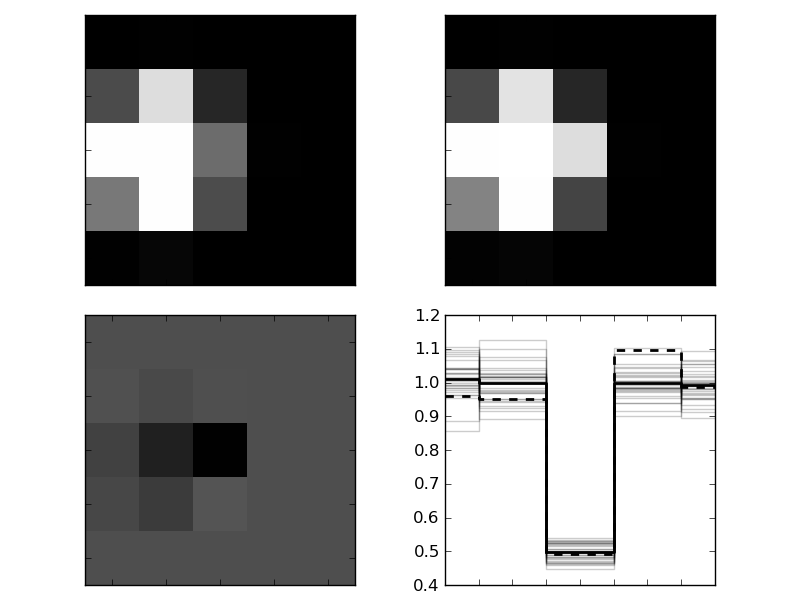
\includegraphics[scale=0.75]{toy32.png}
\caption{A conceptual demonstration of our patch-based,
  self-calibration method.  The top left panel shows a what a $5\times5$
  pixel patch might look like for a high signal to noise (S/N $\sim
  100$) star, after
  calibration with \textsl{calwfc3} (but with no flat field applied).
  The star has a sampling and PSF (at 1.6 microns) that matches WFC3
  (\href{http://bit.ly/XFSb1M}{ISR WFC3 2009-37}).  For this
  illustration, the sensitivity of all the the pixels is set to 100\%
  except for the central pixel, whose sensitivity is reduced by 50\%.
  Next, the top right panel shows what a best-fit model looks like.
  The bottom left shows the difference between the two, where the
  central pixel is clearly inferred to be under-sensitive (given the
  model).  Finally, the bottom right panel show the flat that we would
  infer for the across the row of the central pixel.  The thick dashed
  line is what we get using just the source in the other three
  panels.  The line grey lines are what we get for 32 other stars,
  which fall on random locations inside (or within a few pixels
  outside) the patch.  The thick black line shows the combined flat
  field, inferred from the 32 sources.  While we stress this is a toy
  model for demonstration (real data is less clean, the PSF is less
  well known, and the calibration issues are less severe),
  we note that our AR Calibration project will have
  more sources per pixel.  Additionally, this figure is not making use of
  important prior information (like LP-flats), which we will have for
  all the projects proposed here.}
\label{fig:2D}
\end{figure}



% List here the program numbers and data status for all accepted GO/AR/SNAP
% programs of the PI in at least the last four HST Cycles. Include a list of refereed
% publications resulting from these programs.

%%%%%%%%%%%%%%%%%%%%%%%%%%%%%%%%%%%%%%%%%%%%%%%%%%%%%%%%%%%%%%%%%%%%%%%%%%%

\end{document}          % End of proposal. Do not delete this line.
                                   % Everything after this command is ignored.

